\scanpage{29}
\mspage{15}
\textcircled{9} \uline{Une conjecture} \uline{arithmético-géométrique}

Soient $g,\nu\geq0$ des entiers. On désigne par $\deleted{\unsure{\mathcal T}}M_{g,\nu}$ le topos modulaire 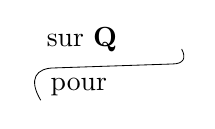
\begin{tikzpicture}[baseline=(base.base)]
\node[anchor=base west,inner sep=0] (base) at (0,0) {pour};
\node[anchor=base west,inner sep=0] at (-0.05,.56) {\inserted{sur $\mathbf Q$}};
\draw[line width=.3pt] (-.12,-.12) .. controls (-.28,.15) and (-.18,.29) .. (.06,.29) -- (1.55,.34) .. controls (1.7,.34) and (1.73,.42) .. (1.67,.53);
\end{tikzpicture} les courbes 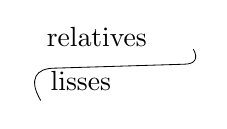
\begin{tikzpicture}[baseline=(base.base)]
\node[anchor=base west,inner sep=0] (base) at (0,0) {lisses};
\node[anchor=base west,inner sep=0] at (-0.05,.56) {\inserted{relatives}};
\draw[line width=.3pt] (-.12,-.12) .. controls (-.28,.15) and (-.18,.29) .. (.06,.29) -- (1.7,.34) .. controls (1.8499999999999999,.34) and (1.88,.42) .. (1.8199999999999998,.53);
\end{tikzpicture} propres relativement connexes de genre $g$, \uline{munies} de \deleted{\unsure{un}} $\nu$-uple de $\nu$ sections disjointes sur chaque fibre

Sauf pour $g=0$, $\nu=0,1,2$ et $g=1$, $\nu=0$, ce topos est associé \unsure{à|:} une étendue algébrique, notion proche = \unsure{schémable}.

On a un hom naturel \deleted{\unsure{extér.}}
\[
\pi_1(\deleted{\unsure{\mathcal T}}M_{g,\nu};\xi)\longrightarrow\operatorname{Autextlac}^{\circ}\bigl(\unsure{\Pi|\pi}_1(\overline X\setminus\{x_1,\mathbin{-},x_\nu\})\bigr)\tag{1}
\]
où $(X;x_1,\mathbin{-}x_\nu)$ $\longrightarrow$ le pt correspondant 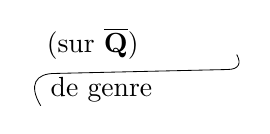
\begin{tikzpicture}[baseline=(base.base)]
\node[anchor=base west,inner sep=0] (base) at (0,0) {de genre};
\node[anchor=base west,inner sep=0] at (-0.05,.56) {\inserted{(sur $\overline{\mathbf Q}$)}};
\draw[line width=.3pt] (-.12,-.12) .. controls (-.28,.15) and (-.18,.29) .. (.06,.29) -- (2.25,.34) .. controls (2.4,.34) and (2.43,.42) .. (2.37,.53);
\end{tikzpicture} $\unsure{g|0}$ avec $\nu$ pts marqués associée à $\xi$ 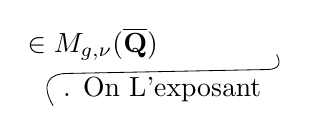
\begin{tikzpicture}[baseline=(base.base)]
\node[anchor=base west,inner sep=0] (base) at (0,0) {. \deleted{On} L'exposant};
\node[anchor=base west,inner sep=0] at (-0.45,.56) {\inserted{$\in M_{g,\nu}(\overline{\mathbf Q})$}};
\draw[line width=.3pt] (-.12,-.12) .. controls (-.28,.15) and (-.18,.29) .. (.06,.29) -- (2.6,.34) .. controls (2.75,.34) and (2.7800000000000002,.42) .. (2.72,.53);
\end{tikzpicture} $\circ$ marque le fait qu'on prend les autom de $\pi_1$ qui n'échangent pas entre eux les classes de lacets associés aux $x_i$\unsure{--|.}
\margin{il faut peut-être être plus strict, et exiger la commutation : des opérations : définies de $\mathfrak S_\nu$ sur le $\pi_1$ ?? Il faut regarder surtout le cas $g=0,\nu=3$....}

Notons qu'on a aussi
\[
\pi_1(\overline M_{g,\nu};\unsure{j|\xi})\longrightarrow\operatorname{Autextlac}^{\circ\circ}\bigl(\unsure{\Pi|\pi}_1(X\setminus\{x_1,\mathbin{-}x_\nu\})\bigr)\tag{2}
\]
où le double $\circ$ indique qu'on prend des autom \inserted{\uline{stricts}} compatibles avec la structure : \unsure{locale|lacets}, \unsure{(i.e.|i.e.} induisant l'identité sur $T=\operatorname{Tate}(\overline{\mathbf Q})$\ldots
\margin{Aut. \unsure{orientés}}
\[
\pi_1(M_{g,\nu}^{an};\unsure{j|\xi})\longrightarrow
\mathrm{Aut}\underbrace{\mathrm{extlac}^{\circ\circ}\unsure{\Pi|\pi}_1(X^{an}\setminus\{}_{\overset{\deleted{\illegible{1}}}{=}\mathcal T_{g,\nu}\ (\text{Teichmüller})}x_1,\mathbin{-}x_\nu\})\tag{2 bis}
\]
dont on sait (théorie top.) que c'est un
\mspage{28}
